


\begin{lemma}
Let $\rDelta$ be a finite set of register updates, where the set of registers contains only one register, and this register is unary.
    \begin{align*}
    \xymatrix{
        \trees \rDelta \ar[r]^f & 
        \text{$\lambda$-terms} \ar[d]^{\text{evaluate}}\\
        \text{unary elements of  $\tmonad \rGamma$} &
        \text{$\lambda$-terms}
    }
    \end{align*}
\end{lemma}
\begin{proof}
    The transformation is described in the following picture:
    \mypic{104}

\end{proof}

\begin{lemma}
    Let $\rDelta$ be a finite set of register updates, over registers $\regnames$ and alphabet $\rGamma$, such that all registers in $\regnames$ are unary. Let $r \in \regnames$.   There exists a finite set $\ranked{\Delta_1}$ of register updates, over registers $\redset r$ and alphabet $\rGamma$,  and a derivable function $f$, such that the following diagram commutes:
        \begin{align*}
        \xymatrix{
            \trees \rDelta \ar[r]^f \ar[d]_{\text{evaluate}}&  
            \trees {\ranked{\Delta_1}} \ar[d]^{\text{evaluate}}\\
            %\text{register valuations over $\regnames$ and $\rDelta$}
            \tmonad \rGamma^{\regnames} \ar[r]_{\text{value of register $r$}} &
            \tmonad \rGamma^{\redset r}
        }
        \end{align*}
    \end{lemma}
    
\newcommand{\reguplambda}{\ranked{\mathrm{regup}_\lambda}}
\begin{align*}
\reguplambda : \text{\ranked{register updates}} \qquad \to \qquad (\tmonad{\rGamma + \set{x, \lambda x, @}} )^{[k]}
\end{align*}
\mypic{106}


The rest of this section is devoted to proving Proposition~\ref{prop:many-register}. To compute its output, first-order tree transducers start with relabeling the nodes of the input tree by register updates following the transition function. Since the later is a first-order tree relabeling, it is derivable thanks to Proposition~\ref{prop:forat}. To show Proposition~\ref{prop:many-register}, it remains to prove that the function
\begin{align*}
\trees(\ranked{\text{Register updates}}) \xrightarrow{\text{Evaluation}} \text{Register valuation} 
\end{align*}
which evaluates a tree of register updates to a register valuation is derivable. For that, we use  terminology inspired by universal algebra, as given in the following definition. 
\begin{definition}
    An \emph{algebra} $\alg$ consists of two sets: 
 \begin{itemize}
 \item a ranked set $\ranked{A}$ called its \emph{domain},
\item  a function $\ranked{A}\cdot A \to A$, called its \emph{shallow product}, 
 \end{itemize}
 where $A$ is the set of nullary elements of $\ranked{A}$. 
    For an algebra $\alg$, define its \emph{product} to be the function of type
    \begin{align*}
\trees( \ranked{A} ) \to A
    \end{align*}
    defined by induction on trees, using the sallow product of the algebra in the natural way.
\end{definition}
Here are some examples of algebras.
\begin{example}[The algebra of register updates] Let $\rGamma$, $\ranked{R}$ be finite ranked
sets. The \emph{algebra of register updates} over $\rGamma$, $\ranked{R}$ is the algebra whose  domain is the ranked set of register updates over output alphabet $\rGamma$ and register names $R$. The nullary elements of the domain are the register valuations.  Its shallow product is the following operation evaluating register updates 
    \begin{align*}
 {\ranked{\text{Register updates}}} \cdot {\text{Register valuations}}  \to \text{Register valuations}
    \end{align*}
The product in this algebra is the operation evaluating a tree of register updates into a register valuation. This  is the operation we are aiming to derive in this section.
\end{example}

\begin{example}[The algebra of (matrix power of) $\lambda$-terms] Let $\Tt$ be a finite set of simple types and $X$ be a finite set of typed variables. 

We define the algebra of $\lambda$-terms $\mathbf{\Lambda X}$, to be the algebra whose domain is $\ranked{\Lambda X}$, the set of $\lambda$-terms over the variables $X$ together with the error type $\ranked{\bot}$, and whose shallow product is the composition of the functions
\begin{align*}
\ranked{\Lambda X}\cdot \Lambda X \xrightarrow{\text{Flatt}} \Lambda X \xrightarrow{\text{Normal form}} \Lambda X 
\end{align*}
where Normal form is the function computing normal form of affine terms using types in $\Tt$ for their sub-terms, and associating $\bot$ to the other terms. 



Now let $k$ be an integer. We set $\mathbf{(\Lambda X)^{[k]}}$ to be the algebra whose domain is the matrix power $\ranked{\mati k {(\Lambda X)}}$, and whose shallow product is the composition of 
\begin{align*}
\ranked{(\Lambda X)^{[k]}}\cdot (\Lambda X)^{[k]} \underset{\text{unfold}}{\xrightarrow{\text{Shallow}}} (\ranked{\Lambda X}\cdot \Lambda X)^{[k]}  \xrightarrow{(\text{Product of }\mathbf{\Lambda X})^{[k]}} (\Lambda X)^{[k]} 
\end{align*}

Thanks to Theorem~\ref{thm:normalise} and ~\ref{thm:stt}, the product of $\mathbf{(\Lambda X)^{[k]}}$ is derivable, as the composition of the following derivable functions
\begin{align*}
\trees(\ranked{\Lambda X})^{[k]} \xrightarrow{\text{Unfold}} (\trees \ranked{\Lambda X})^{[k]} \xrightarrow{\text{flatt}^{[k]}} 
 (\Lambda X)^{[k]} \underset{\text{form}}{\xrightarrow{\text{Normal}}}  (\Lambda X)^{[k]}
\end{align*}
\end{example}

To show that an algebra has a derivable product, we will be to embed it into another algebra whose 
product is known to be derivable. This justifies the following definition.

Let $\mathbf{A}$, $\mathbf{B}$ be two algebras. An \emph{embedding} of $\mathbf{A}$ into $\mathbf{B}$ is a function $\ranked{f: \ranked{A}\to \ranked{B}}$ which makes the following diagram commutes ($f$ is the restriction of $\ranked{f}$ to $A$.)
      \begin{align*}
    \xymatrix@C=2cm{
        \ranked{A} \cdot A \ar[r]^{\ranked{f}\cdot f} \ar[d]_{\text{Shallow product}} & \ranked{B}\cdot B \ar[d]^{\text{Shallow product}}\\
A \ar[r]_{f} & B       
       }
    \end{align*} 
It is easy to check that the following diagram also commutes for embeddings    
        \begin{align*}
    \xymatrix@C=2cm{
        \trees(\ranked{A}) \ar[r]^{\trees(\ranked{f})} \ar[d]_{\text{Product}} & \trees(\ranked{B}) \ar[d]^{\text{Product}}\\
A \ar[r]_{f} & B       
       }
    \end{align*}  
 In the light of this property, to show that the product of an algebra $\mathbf{A}$ is derivable, it is enough to find an algebra $\mathbf{B}$ and an embedding $\ranked{f}$ of $\mathbf{A}$ into $\mathbf{B}$ such that: $\ranked{f}$ is derivable,  the product of $\mathbf{B}$ is derivable, $f$ is invertible and its inverse $f^{-1}$ is derivable.  

In our case, we will embed the algebra of register updates into an algebra $\mathbf{(\Lambda X)^{[k]}}$, for a well chosen set of variables $X$ and set of types $\Tt$. As noticed earlier, the product of the latter is derivable, we only need to show that the additional derivability conditions on the embedding.

Let us fix a register transducer with output alphabet $\rGamma$ and a set $R$ of $k$ register names. 
We suppose without loss of generality that all registers are unary\footnote{We can always encode the content of an $n$-ary register by several unary registers.}. Let $X$ be the set of variables 
\begin{align*}
X  \quad \eqdef \quad \set{\typevar {x_a} {\otype^i \to \otype} : a \in \rGamma \text{ of arity $i$}} \cup \set{\typevar {x} \otype}.
\end{align*}
and $\Tt$ be the set of simple types 
\begin{align*}
    \Tt \quad \eqdef \quad \set{\otype^i \to \otype : i \in \set{0,\ldots,\text{maximal arity of $\rGamma$}}}
\end{align*}
We define the function $\ranked{f}$ from the algebra of register updates over $\rGamma$, $\ranked{R}$ to  the algebra $\mathbf{\Lambda X}$ as in the following picture
\begin{center}
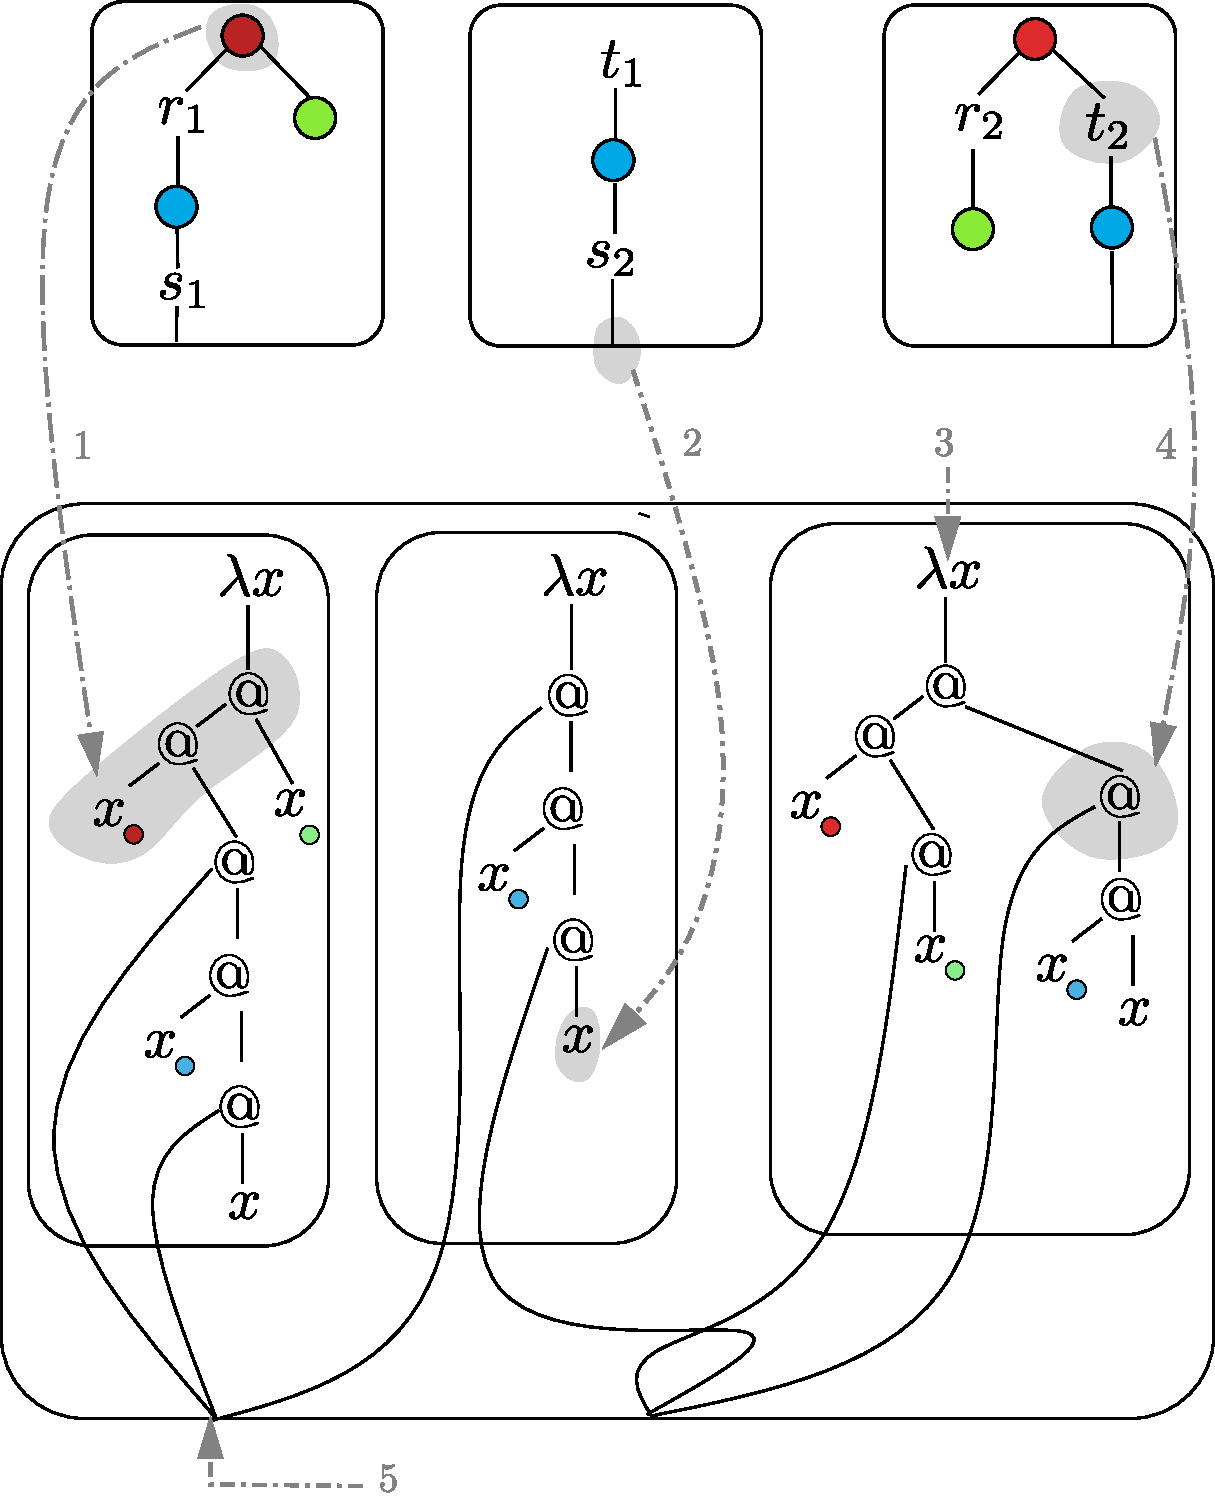
\includegraphics[scale=.4]{embedding.pdf}
\end{center}
\begin{enumerate}
\item Every $n$-ary symbol $a$ of $\rGamma$ is replaced by a spine of $@$ nodes of lenght $n$ ending by the variable $x_a$.
\item Ports of register updates become the variable $x$.
\item A node $\lambda x$ is added as a root of every register update.
\item Register names become an $@$ node whose left child is a port. 
\item Ports coming from the same copy of name registers are folded in the same port. The order of the fold respects registers order.
\end{enumerate}
